%-*-texinfo-*-
%This is part of the "UFO:Alien Invasion"-Reference Manuals Tex sources.
%Copyright (C) 2006 Eric Goller.
%See the file ufo-manual_EN.tex for copying conditions.

\chapter{Tactical combat - Battlescape}

\section{Battlescape - an overview}
So this is where all the fun happens ;) It is here that you former choices have to proof their worth as well as you will have to prove your commanding skills.

The goal of every tactical combat is quite simple: kill all those evil aliens with as few civilian (and of cause squad) looses as possible. In order to achieve this you will have to find a good balance between caution and fast proceedings. You don't want all you soldiers...

In the course of the game you will see a wide range of settings and environments, but no matter how bad things might look like, there a some quite powerfull tools at you hand to get rid of them. The main task of the following section is to get familiar with most of them. If you have some experience with (turn-based) tactical combat games you should find some redundant elements - and of cause you will if you ever played any other UFO before. Nevertheless you should take a short overview over the interface so you make sure you don't miss any important feature.

\subsection{Buttons}
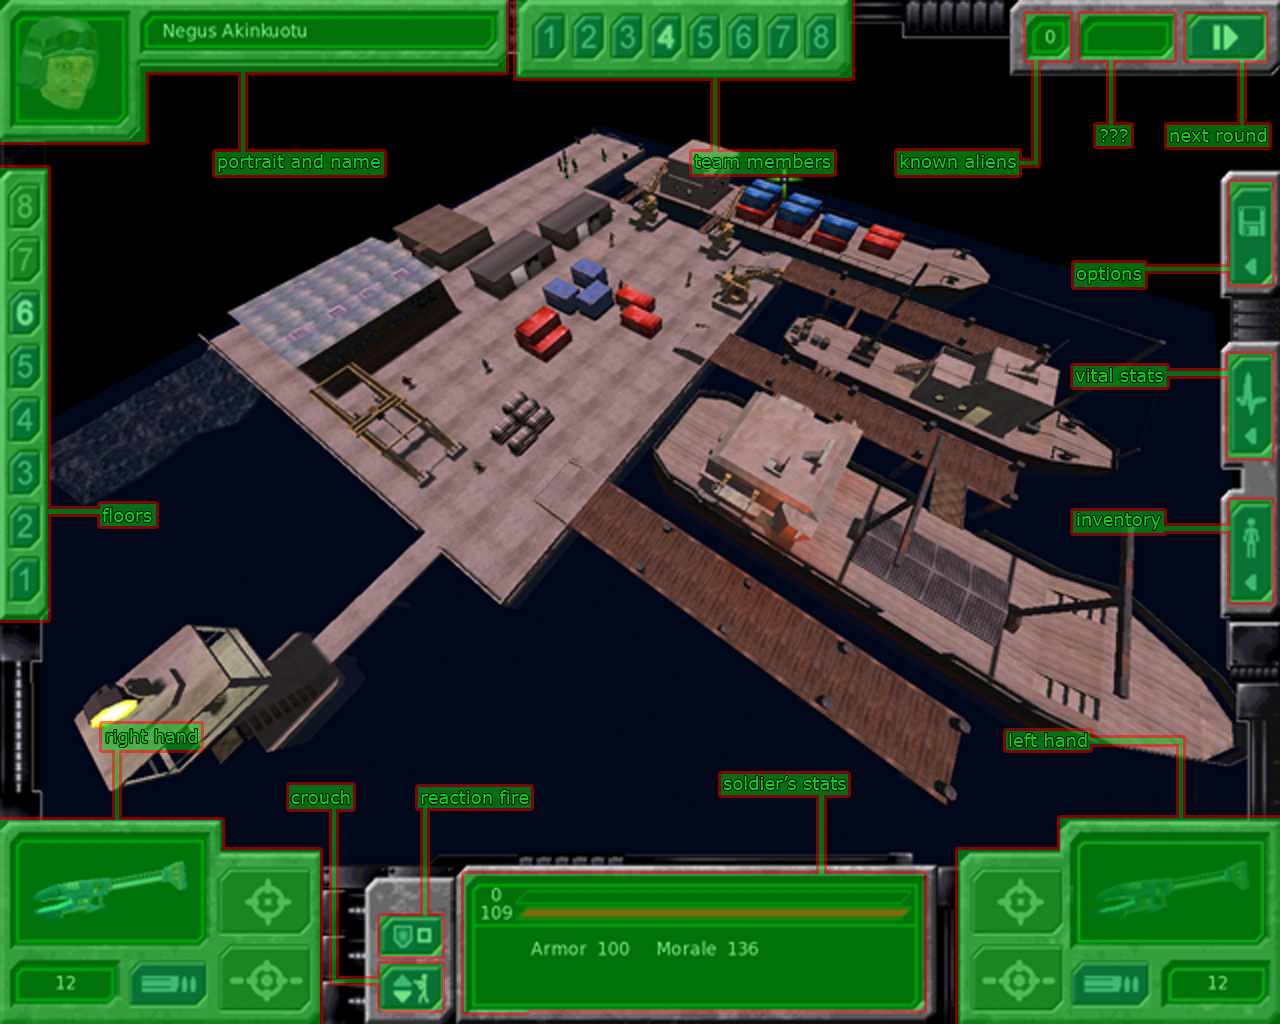
\includegraphics[width=\textwidth]{images/HQ/tactical_overview_finalHQ.jpg}
\paragraph*{Floors}
Here you can change the "ground-level" or floor shown in the tactical view. Besides its obvious use in order to move you soldiers between different floor-levels its also helpful to get an general overview. So it's always a smart move to switch between all levels at the beginning of each mission so you won't miss the "hidden" cellar or rooftop.
\paragraph*{Portrait and name}
This is more for astheticl reasons, so no big actions are bound to this. (But of cause - as usual- suggestions are welcome)
\paragraph*{Team-members}
There is where you can switch between you soldiers (alternatively use keybindigs: 1 to 8 / just left-click on their model). In case one (or more *G*) of your devoted fighters lost his live fighting the evil his button will become gray.
\paragraph*{Known aliens}
This states the number of aliens all your squad member have discovered this round. By clicking on it you may switch through all of them.
\paragraph*{???}
\textbf{I don't have a glue what this is for. Maybe someone wants to give me a hint... ? ;)}
\paragraph*{next round}
Hmm... so what do you suspect this one does ? Exactly !
\paragraph*{Options}
Opens the "Options"-menu where you may vary several video/sound-settings as well as aboard or retry current missions. Be aware that it's not possible nor intended to save a ongoing mission.
\paragraph*{Vital stats}
This is where you find more detailed information about health, moral and psi-power of your soldier.
\paragraph*{Inventory}
Opens the inventory of the selected soldier. This is where you can change weapons, pick up/drop items or just take a look at your great heros.
\paragraph*{Soldiers stats}
This is a summery of all general information you need to use your soldier most efficently. Its content interacts with your mouse action, but should be quite self-explaining. Not only you will find health and remaining TUs (we will deal with TUs in the following section) here but also it will give you the amount your currently selected shooting-mode will consume as well as some other infos like current armor and moral.
\paragraph*{Reaction fire}
This button enables "reaction fire" a central concept of every tactical combat. We will deal with it in the following chapter. For now you should just remember that it is here where you turn it on and off.
\paragraph*{Crouch}
As one might guess, this button will make your soldier kneel down (and by doing so reduceing the danger of beeing hit by enemy fire) or if he already does make him stand up. Please notice that a soldier that kneels down can still move forward as if he would stand upright, but it takes him 1 additional time unit per square to do so.
\paragraph*{Right/left-hand}
Those two fields are completely identical besides the fact the left hand one is active only if you actualy wear two one-handed items/weapons. If you have a two-handed item/weapon equiped the left-hand field will be inactive. Because each of the two fields consist of several important buttons itself we will discuss them a bit more detailed. Please take a look at the following image.
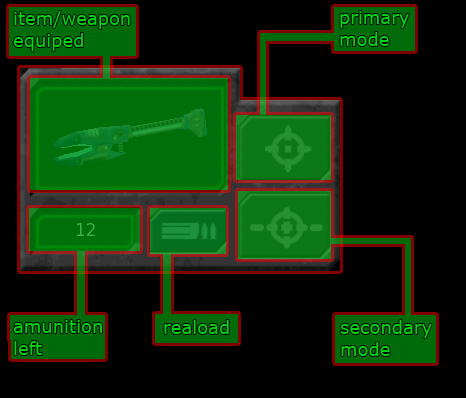
\includegraphics[width=6cm]{images/HQ/weapon_buttons_finalHQ.jpg}
%als float ?!
\subparagraph*{Item/weapon}
Gives a picture of the currently equiped item/weapon. This turnes red in case you can't use the weapon, for example because you don't know the tech or don't have any ammunition left.
\subparagraph*{Primary-mode}
Activates primary-mode for this item. In case of weapons this is usualy (but not always!) a fast but less accurate / powerfull shoot. For Details see weapon discription.
\subparagraph{Secondary-mode}
Activates secondary-mode for this item. In case of weapons this is usualy (but again, not always!) a more TU-consuming but also more accurate / powerfull shoot. Please notice that in case the item supports only one mode (like stun rod) both modes are identical.
\subparagraph*{Reload}
Reloads currently equiped weapon, if ammunition is left in the inventory.
\subparagraph{Amunition left}
Shows the amunition left in your weapon. Please notice that some shooting-modes (also some of the one-shoot ones) require more than one "bullet" here.

\subsection{What to do now ... ?}
%da selbsterkl�rend und wenig untermen�s kurz halten
\section{Game-mechanics (Battlescape)}
\subsection{Time-units (TUs)}
As mentioned before every soldier has a certain amount of time units (TUs) which are mainly determined by his "speed" attribute. Every action done by him costs him a varing amount of TUs this holds for firing or reloading a weapon as well as walking or reequiping him in the inventory. The amount of TUs needed for using the primary/secondary mode is given in the status window after selecting one of the two.

\subsection{Movement}
Like firing a weapon, movement also consumes time units. You can make your soldier walk to a spot using your mouse on the tactical view. You will notice that your cursor turns to a green square indicating that this place is reachable with your current amount of TUs or turn blue if it is not (this might be the case due to a lack of TUs or for geographical reasons). If the square is green it will also prompt two numbers of which the first one states the TU-cost of this movement while the second one represents your actual amount of TUs. In case your soldier notices a new enemy or civilian in his line of sight while walking the movement will be interrupted, giving you the chance to adjust your orders according to this new situation.

\subsection{Shooting}
\subsubsection{Line of sight}
For obvious reasons you soldiers, in general, can only shoot at what they do see. After finishing an ordered movement your soldier will look in the direction of his last step, which is not very helpful in a lot of situations. To solve this you might make use of the possibility to change your soldiers viewing direction. This can be done in different ways, eg. 3rd-mouse-button / ctrl.-button/ q-button. For details please refer to your keybindigs. 
\subsubsection{Shooting-modes}
As we have said before most items, weapons in particular, do have two different action/firing-modes. While the second firing-mode of a sniper rifle is an aimed shot, some assault rifles can start a long fireburst or fire one concentrated and by that devastating single beam. Whatever weapon raises you interest, Ufopedia is your friend. Using the integrated[\textbf{will this be up in RC5?} Ufopedia links you will get to the according entry by simply right-clicking on it. If you look up a certain weapon like that you might be confused, the only information that can be found here is its name and if its a twohanded one or not. What seems rather wired on first sight has a simple reason. As some weapons can be equiped with a wide range of different kinds of ammunition their use and stats also heavily depend on the amunition loaded. So once you look up the amunition you want to use you will find all the data and statistics you are looking for - given you have done the required research. Doing so you will find that different firing-modes not only differ by TU needed and damage done but also by weapon skills needed.
\subsubsection{Chance to hit}

\textbf{Do we want to give details about CtH calculation to the player ? Well, the display for it (while aiming at a target) seems buggy yet anyway... at least for me ;)}

\subsubsection{Close combat }
An alien is poping up just around the corner and not enough TUs left to fire this Plasma-Blaster in secondary mode while primary-mode offers only indirect fire? Your soldiers beeing keen on some extra thrill ? You want to capture an living alien for "interogation"   but all your research department has to offer is a stun rod of which they say it might work - somehow... ? No matter what the reason may be, there will be a time you will get into close-combat, or it will get to you. While the reason to be that close to an hostile alien might be quite scary, luky enough the way to use the interface in such a situation is not at all. Overall it works exactly like caring a gun besides the fact that your power skill is taken into consideration when calculating the combat results.\textbf{is it like that ? shouldn't it be ?} Also most close combat weapons (that includes pistols as well) do have a far more devastating impact on their target compared for their needed TUs making them a reasonable choice in small and narrow enviroments like buildings and the likes.

\subsubsection{Friendly fire}

\textbf{is the current situation a bug or a wanted feature ? making FF almost as lethal to every squadmember as any alien could be} 

\subsubsection{Reaction fire}
One of the main aspects every experienced commander needs to be able to use for his advantage is what is called "reaction-fire"(RF). When discussing the basics of battlescape we already mentioned its button but spared to explain the corresponding concept. When enabled (costing a certain amount of TUs) your soldier will be able to react on new situations and sightings after you already ended your turn. For doing so he has all the TUs left from your current turn plus half of the upcoming turns TUs at his disposal. So whenever an enemy gets into (or already is) the line of sight of our brave hero he will use those TUs at his disposal to fire his weapon in order to deal with this more or less suprising situation. So in order to get the most of it and make your soldier really kill an alien it might be a smart move not to leave him with RF activated but no further TUs at his hand - which would leave him with only 50\% of the upcoming turns TUs for his answer to an enemy poping up. Somtimes, especially after having suffered heavy penetration by enemy fire with reaction-fire activated, your soldiers will refuse your order to "turn it off" as they are too scared to let their guard down. For details about this and other effects of a bad moral please refer to the according section of the manual.
\textbf{select weapon for RF ?!}

\subsubsection{Damagetypes}
\textbf{we dont have anything concrete to be put here or ? If we do, pls let me know... :)}

\subsubsection{Stun}
\textbf{as i don't know how far implementation is done yet i will only sketch it for now}
In order to find out more about your alien enemy and his goal, motivation and structures you might find it usefull to catch one or more them for direct interrogation. Once your research lab developed the tools needed to do so you might use them as any other weapon of this kind (e.g. grenades, close-combat, etc.). After successfuly finishing a mission those stuned alien will be brought to your base. Please be aware that you will need special structures to make sure your "guest" will stay long enough to give you any answer at all. If you lack those facilities your stuned aliens will die instantly once you reach your inproper base.\textbf{at least that's the plan ?!} In case everything is prepared to make your stuned aliens feel home they will open up new options in the research department.

\subsection{moral}
\textbf{i don't have any infos about this one. once again if someone has I would be glad as there seems to be some kind of implemention done already}
\section{Tips and Hints}
%evtl. Teile der Spielmechanik hierher !?
\textbf{suggestions welcome / obsoleteable}